\documentclass{beamer}

\mode<presentation> {
\usetheme{Madrid} %Default - Use this
\usecolortheme{whale}
}

%%%%%%%%%%% To Set the reference to black color (Default is blue color for this theme )
\setbeamertemplate{bibliography item}[text] % For IEEE Format citations
\setbeamercolor{bibliography item}{fg=black} 
\setbeamercolor{bibliography entry author}{fg=black}
\setbeamercolor{bibliography entry title}{fg=black} 
\setbeamercolor{bibliography entry location}{fg=black} 
\setbeamercolor{bibliography entry note}{fg=black}


\usepackage{graphicx}
  \DeclareGraphicsExtensions{.pdf,.jpeg,.png,.eps,.jpg}
\usepackage{booktabs} % Allows the use of \toprule, \midrule and \bottomrule in tables
\usepackage{multirow} % For multirow table
\usepackage{amssymb,amsmath,bm}
\usepackage{amsmath}
\usepackage[para]{threeparttable}


%\usepackage{fancyvrb} % For verbatim
%\usepackage{fixltx2e}

%\usepackage[font=Helv,timeinterval=10]{tdclock}
%\setbeamertemplate{headline}{\initclock\tiny{\cronominutes\pdfcolon\cronoseconds}}


%----------------------------------------------------------------------------------------
%	TITLE PAGE
%----------------------------------------------------------------------------------------

\title[First Seminar]{Multi-stage Children Story Speech Synthesis} 

\author[Harikrishna D M]{
{\footnotesize{First Seminar} \\ 
{\textit{by}} \\ 
\textbf{{Harikrishna D M}} \\
{Roll No. 12IT72P07}\\ \vspace*{3mm}
%\begin{figure}
\includegraphics[width=0.1\linewidth]{figures/iit_kgp_80} \\ \vspace*{3mm} % For Blue Color
%\includegraphics[width=0.1\linewidth]{figures/iitlogo} \\ \vspace*{3mm} % For Black Color
%\end{figure}
{\textit{under the supervision of}}\\ \vspace*{2mm}
\textbf{{Dr. K. Sreenivasa Rao}} \\ \vspace*{1mm}
{\bf{School of Information Technology\\ Indian Institute of Technology Kharagpur}}
}
}

\date{August 6, 2015} % Date, can be changed to a custom date


\begin{document}

\begin{frame}
\titlepage % Print the title page as the first slide
\end{frame}

\begin{frame}
\frametitle{Overview} 
\tableofcontents 
\end{frame}

%----------------------------------------------------------------------------------------
%	PRESENTATION SLIDES
%----------------------------------------------------------------------------------------

%%%%%%%%%%%%%%%%%%%%%%%%%%%%%%%%%%%%%%%%%%%%%%%%%%%%%%%%%%%%%%%%%%%%%%%%%%%%%%%%%%%%%%%%%
\section{Introduction} \label{Introduction}


\begin{frame}
\frametitle{Introduction}
\begin{itemize}

\item[--] Synthesizing expressive speech: Embedding natural expressions into speech, according to the semantics present in the text.
\item[--] Story synthesis: Synthesizing story-style speech from the text using text-to-speech (TTS) systems. 
\item[--] Story synthesis approaches 
\begin{itemize}
\item[--] Development of TTS systems using story speech corpus.
\item[--] Rule-based story speech synthesis.
\end{itemize}

\item[--] Application: Audiobooks.

\end{itemize}


\end{frame}
%%%%%%%%%%%%%%%%%%%%%%%%%%%%%%%%%%%%%%%%%%%%%%%%%%%%%%%%%%%%%%%%%%%%%%%%%%%%%%%%%%%%%%%%%





\section{Literature Review}

%%%%%%%%%%%%%%%%%%%%%%%%%%%%%%%%%%%%%%%%%%%%%%%%%%%%%%%%%%%%%%%%%%%%%%%%%%%%%%%%%%%%%%%%%
\begin{frame}
\frametitle{Literature Review: Text Classification}

\begin{table}[h]
\renewcommand{\arraystretch}{1}
\caption {Literature Review in the context of Text Classification \label{Table: Text Classification}} 
\vspace{-0.35cm}
\resizebox{\linewidth}{!}{
\begin{tabular}{|p{2.5cm}|p{4cm}|p{3.5cm}|p{5cm}|}
\hline
Author & Work & Dataset & Contribution \\ \hline

Joachims (1998) \cite{joachims1998text} & Text categorization with SVM & Ohsumed (Medical abstracts): 13929 documents, 23 classes & Use of SVM for text classification  \\ \hline

Yang et al. (1999) \cite{yang1999re} & Examination of text categorization methods & Reuters (News articles): 21578 documents, 90 classes & Controlled study with statistical signicance tests: SVM, KNN, NN, LLSF and NB \\ \hline

Moldovan et al. (2005) \cite{moldovan2005latent} & LSA for patent documents & USPTO (Patent documents): 33923 documents, 10 classes & Comparison of VSM and LSA \\ \hline

Sainath et al. (2010) \cite{sainath2010sparse} & Sparse representation for text classification & 20 Newsgroup (News articles): 20000 documents, 20 classes & Slight improvement in SR method over NB \\ \hline

\end{tabular}}
\end{table}	

\begin{itemize}
\item[--] Limited to text classification in the domains such as news articles, medical abstracts and patents.
\end{itemize}

\end{frame} 
%%%%%%%%%%%%%%%%%%%%%%%%%%%%%%%%%%%%%%%%%%%%%%%%%%%%%%%%%%%%%%%%%%%%%%%%%%%%%%%%%%%%%%%%%



%%%%%%%%%%%%%%%%%%%%%%%%%%%%%%%%%%%%%%%%%%%%%%%%%%%%%%%%%%%%%%%%%%%%%%%%%%%%%%%%%%%%%%%%%
\begin{frame}
\frametitle{Literature Review: Story-telling Applications}

\begin{table}[h]
\renewcommand{\arraystretch}{0.9}
\caption {Literature Review in the context of Story-telling Applications \label{Table: Story-telling Applications}} 
\vspace{-0.35cm}
\resizebox{\linewidth}{!}{
\begin{tabular}{|p{2cm}|p{3.5cm}|p{4.5cm}|p{4.5cm}|}
\hline
Author & Work & Contribution & Result \\ \hline
Alm et al. (2005) \cite{alm2005perceptions} & Perceptions of emotions in expressive storytelling & Analysis of expressive story-telling speech & Semantic and prosodic cues collaborate to express and reinforce emotional content \\ \hline 

Lobo et al. (2010) \cite{lobo2010fairy} & Fairy tale corpus organization & LSA to represent stories, and recommendation algorithm to define clusters of similar stories & Organized 453 fairy tales from Project Gutenberg \\ \hline
Ceran et al. (2012) \cite{ceran2012semantic} & A semantic triplet based story classifier & $<Subject, Verb, Object>$ triplets to identify paragraph as story or not & Better performance with keyword, POS, named entities and semantic triplet features \\ \hline
Iosif et al. (2014) \cite{iosif2014speaker} & Multi-step system for children story analysis & Character identification, attribution of quotes and affective analysis of quoted materials & Hybrid approach for children story analysis \\ \hline

\end{tabular}}
\end{table}	

\begin{itemize}
\item[--] Limited to corpus organization, story analysis and identification.
\end{itemize}

\end{frame} 
%%%%%%%%%%%%%%%%%%%%%%%%%%%%%%%%%%%%%%%%%%%%%%%%%%%%%%%%%%%%%%%%%%%%%%%%%%%%%%%%%%%%%%%%%



%%%%%%%%%%%%%%%%%%%%%%%%%%%%%%%%%%%%%%%%%%%%%%%%%%%%%%%%%%%%%%%%%%%%%%%%%%%%%%%%%%%%%%%%%
\begin{frame}
\frametitle{Literature Review: Indian Languages}

\begin{table}[h]
\renewcommand{\arraystretch}{1}
\caption {Literature Review in the context of Indian Language \label{Table: Literature Indian Languages}} 
\resizebox{\linewidth}{!}{
\begin{tabular}{|p{1.5cm}|p{2.5cm}|p{3cm}|p{3cm}|p{3cm}|}
\hline
Language & Author & Work & Contribution & Result \\ \hline
Punjabi & Nidhi et al. (2012) \cite{nidhi2012domain} & Classification of Punjabi news articles & Sports specific ontology, Gazetteer lists & Ontology Based Classification $>$ NB  \\ \hline
Marathi & Meera et al. (2014) \cite{game2014comparison} & Comparison of Marathi text classifiers & Rule based stemmer and Marathi word dictionary & NB $>$ Centroid $>$ Modified KNN $>$ KNN  \\ \hline
Kannada & Deepamala et al. (2014) \cite{deepamala2014text} & Kannada Webpage Classification & Sentence boundary detection, stemming, stopword removal & Performance improvement with stemming and stopword removal \\ \hline
\end{tabular}}
\end{table}	

\end{frame} 
%%%%%%%%%%%%%%%%%%%%%%%%%%%%%%%%%%%%%%%%%%%%%%%%%%%%%%%%%%%%%%%%%%%%%%%%%%%%%%%%%%%%%%%%%


%%%%%%%%%%%%%%%%%%%%%%%%%%%%%%%%%%%%%%%%%%%%%%%%%%%%%%%%%%%%%%%%%%%%%%%%%%%%%%%%%%%%%%%%%
\begin{frame}
\frametitle{Literature Review: Indian Languages (Cont..)}

\begin{table}[h]
\renewcommand{\arraystretch}{1}
\caption {Literature Review in the context of Indian Language \label{Table: Literature Indian Languages}} 
\resizebox{\linewidth}{!}{
\begin{tabular}{|p{2cm}|p{2.5cm}|p{3.5cm}|p{3.5cm}|p{3.5cm}|}
\hline
Language & Author & Work & Contribution & Result \\ \hline
Tamil & Rajan et al. (2009) \cite{rajan2009automatic} & Tamil document classification & Comparison of VSM and ANN & ANN $>$ VSM  \\ \hline
Telugu & Kavi Narayana Murthy (2003) \cite{murthy2003automatic} & Telugu News Articles classification & Used NB to classify news articles into Politics, Sports, Business and Cinema
 & Base system for telugu document classification  \\ \hline
Ten Indian Languages & Raghuveer et al. (2007) \cite{raghuveer2007text} & Text Categorization in Indian Languages using ML Approaches & Corpus-based machine learning techniques for text categorization & SVM outperformed KNN and NB \\ \hline

\end{tabular}}
\end{table}	

\begin{itemize}
\item[--] Limited to text classification in the domains such as news articles and web pages.
\item[--] None of the works attempted story classification in Indian languages
\end{itemize}

\end{frame} 
%%%%%%%%%%%%%%%%%%%%%%%%%%%%%%%%%%%%%%%%%%%%%%%%%%%%%%%%%%%%%%%%%%%%%%%%%%%%%%%%%%%%%%%%%


\section{Scope of the work}


%%%%%%%%%%%%%%%%%%%%%%%%%%%%%%%%%%%%%%%%%%%%%%%%%%%%%%%%%%%%%%%%%%%%%%%%%%%%%%%%%%%%%%%%%
\begin{frame}
\frametitle{Scope of present work}
\begin{itemize}
\item[--] Highly challenging task: Generating an expressive, naturally sounding, story like speech from text using a neutral TTS system. 
\item[--] Steps in story synthesis
\end{itemize}
\begin{figure} 
\centering
\resizebox{7cm}{4cm}{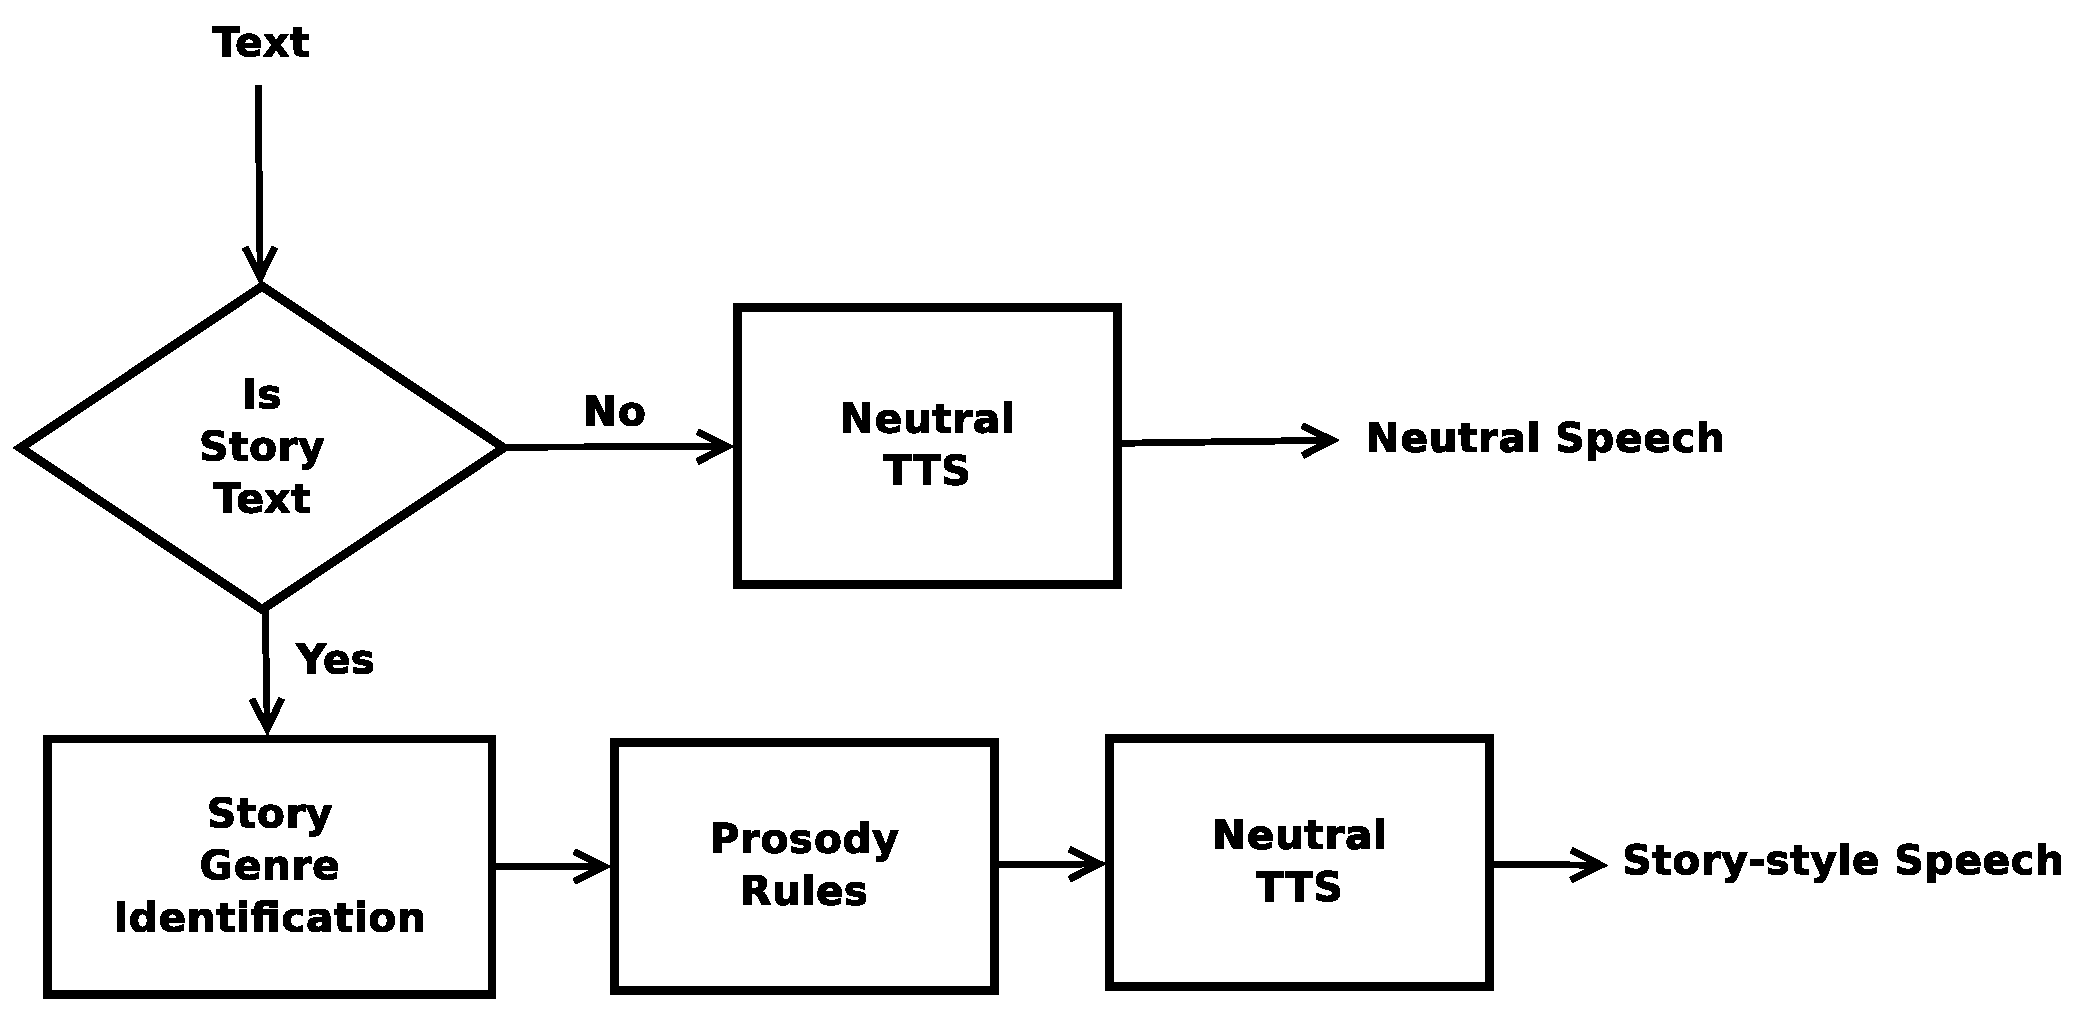
\includegraphics{figures/Objective_1}}
\centering
\caption{Overview of steps in story synthesis}
\label{system}
\end{figure}
\end{frame}
%%%%%%%%%%%%%%%%%%%%%%%%%%%%%%%%%%%%%%%%%%%%%%%%%%%%%%%%%%%%%%%%%%%%%%%%%%%%%%%%%%%%%%%%%

%\item[--] Input: \href{run:Story.txt}{Story Text} %%%%% Use This %%%%%
%\item[--] Neutral TTS System: \href{run:Neutral.wav}{TTS Output} %%%%% Use This %%%%%
%\item[--] Desired Output: \href{run:Story.wav}{Story Style Speech} %%%%% Use This %%%%% 

%%%%%%%%%%%%%%%%%%%%%%%%%%%%%%%%%%%%%%%%%%%%%%%%%%%%%%%%%%%%%%%%%%%%%%%%%%%%%%%%%%%%%%%%%

\begin{frame}
\frametitle{Motivation}
\begin{itemize}
\item[--] Project requirement: \textit{“Development of Text-to-Speech systems in Indian languages (Phase - II)”.}
\item[--] Basic objective: To synthesize story style speech from a story text using the neutral text-to-speech (TTS) systems developed in $Phase - I$ of the project.
\item[--] Demo: \href[pdfnewwindow]{run:Story.pdf}{\beamergotobutton{Story Text}}  \href{run:Neutral.wav}{\beamergotobutton{Neutral TTS Output}} \href{run:Story.wav}{\beamergotobutton{Desired Story Style Speech}}
\item[--] Syllable-based unit selection neutral TTS systems developed for six Indian languages in Phase - I of the project \cite{patil2013syllable}.
\item[--] Each story will be narrated in different style depending on story type.
\item[--] Derivation of story specific prosody rules.
\item[--] Attempting story classification in view of synthesizing story speech.
\end{itemize}
\end{frame}

%%%%%%%%%%%%%%%%%%%%%%%%%%%%%%%%%%%%%%%%%%%%%%%%%%%%%%%%%%%%%%%%%%%%%%%%%%%%%%%%%%%%%%%%%

	
%%%%%%%%%%%%%%%%%%%%%%%%%%%%%%%%%%%%%%%%%%%%%%%%%%%%%%%%%%%%%%%%%%%%%%%%%%%%%%%%%%%%%%%%%

\section{Work Done}

\begin{frame}
\frametitle{Work Done}
\begin{itemize}
\item[--] Story Classification Framework 
\item[--] Story Classification using Keyword based Features 
\item[--] Story Classification using POS Features 
\item[--] Story Classification using Concatenation of Keyword and POS Features 
\end{itemize}
\end{frame}

%%%%%%%%%%%%%%%%%%%%%%%%%%%%%%%%%%%%%%%%%%%%%%%%%%%%%%%%%%%%%%%%%%%%%%%%%%%%%%%%%%%%%%%%%
\begin{frame}
\begin{center}
\Huge{Story \\Classification \\Framework}
\end{center}
\end{frame}
%%%%%%%%%%%%%%%%%%%%%%%%%%%%%%%%%%%%%%%%%%%%%%%%%%%%%%%%%%%%%%%%%%%%%%%%%%%%%%%%%%%%%%%%%

%%%%%%%%%%%%%%%%%%%%%%%%%%%%%%%%%%%%%%%%%%%%%%%%%%%%%%%%%%%%%%%%%%%%%%%%%%%%%%%%%%%%%%%%%
\begin{frame}
\frametitle{Story Classification Framework}
\begin{figure} 
\centering
\resizebox{8cm}{6cm}{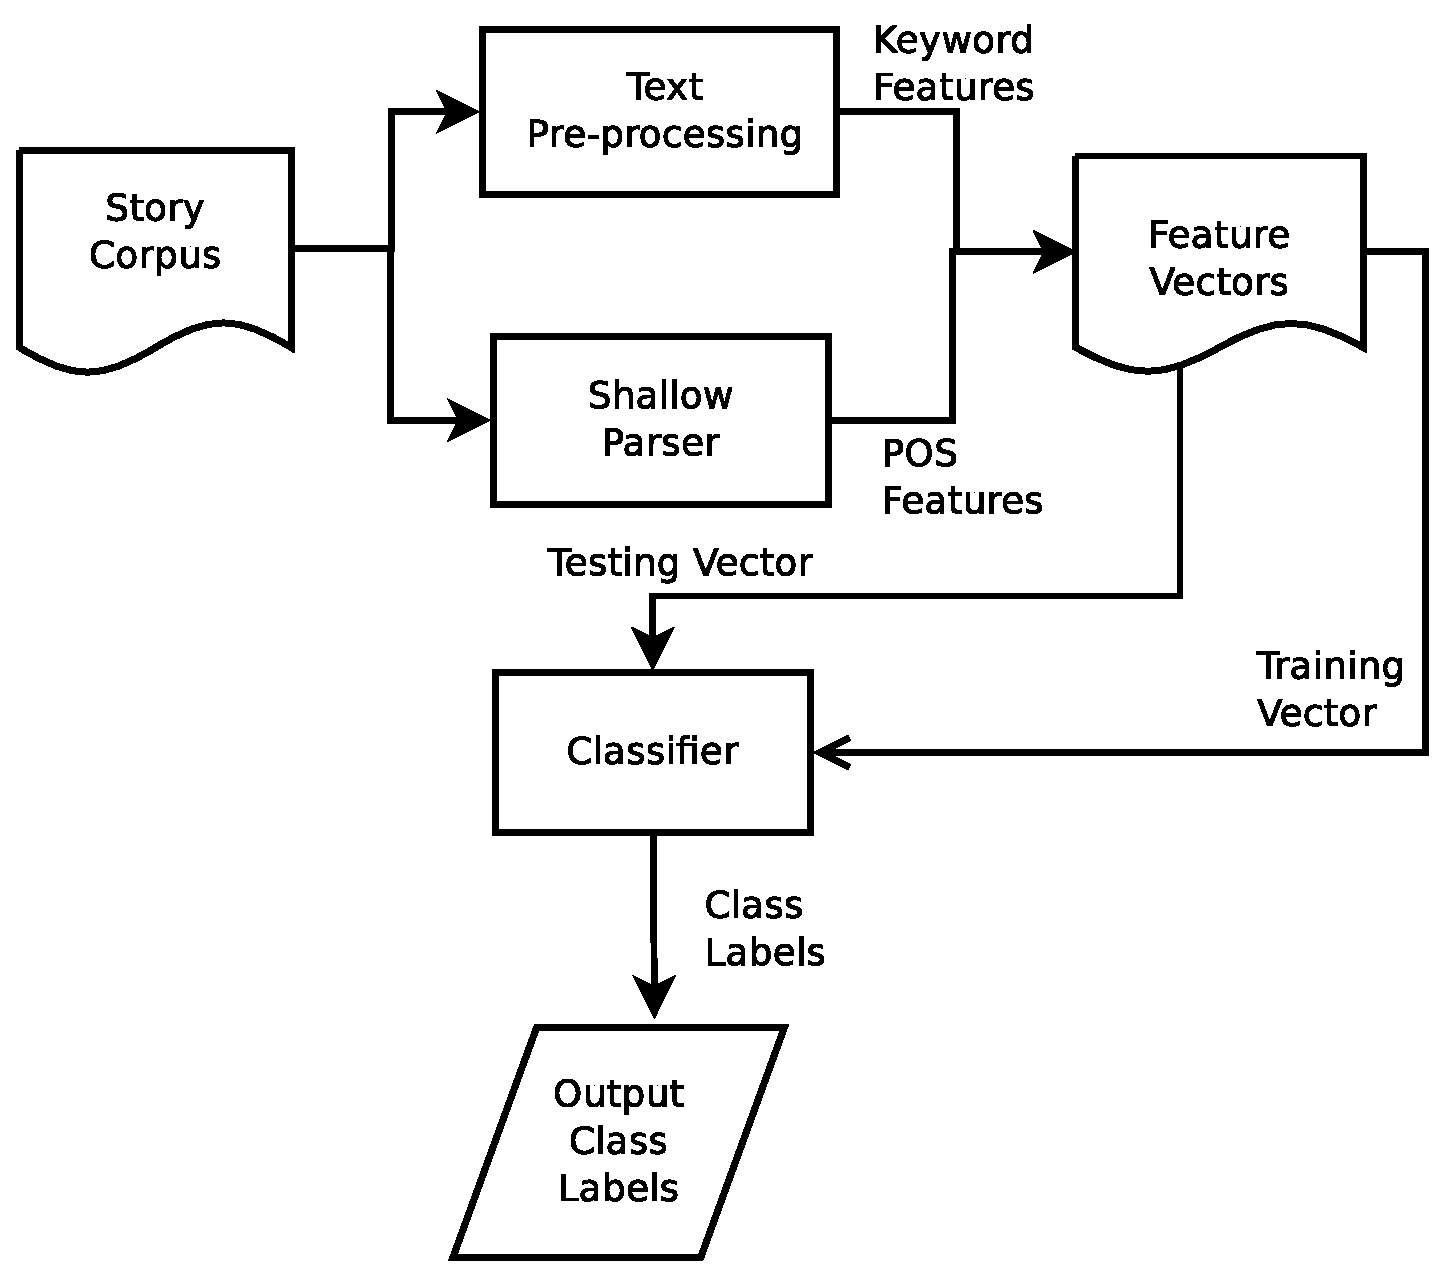
\includegraphics{figures/system}}
\centering
\caption{Flow diagram of Story Classification Framework}
\label{system}
\end{figure}
\end{frame}
%%%%%%%%%%%%%%%%%%%%%%%%%%%%%%%%%%%%%%%%%%%%%%%%%%%%%%%%%%%%%%%%%%%%%%%%%%%%%%%%%%%%%%%%%

%%%%%%%%%%%%%%%%%%%%%%%%%%%%%%%%%%%%%%%%%%%%%%%%%%%%%%%%%%%%%%%%%%%%%%%%%%%%%%%%%%%%%%%%%
\begin{frame}
\frametitle{Story Corpora}
\begin{itemize}
\item[--] Hindi and Telugu story corpora: 300 and 150 short stories from Blogs\footnote{http://telugubalalu.blogspot.in/}, Panchatantra and Akbar-Birbal books.  
\item[--] Classification of stories into three genres: Fable, folk-tale and legend.
\item[--] Definition of story genres
\begin{itemize}
\item[--] Fable: Tale involving animals as an essential character.
\item[--] Folk-tale: Story passed on from one generation to the next. 
\item[--] Legend: Story carrying significant meaning or symbolism for the culture.
\end{itemize}
\end{itemize}

\begin{table}[h]
\renewcommand{\arraystretch}{1}
\footnotesize\setlength{\tabcolsep}{8pt}
\caption {Details of Hindi and Telugu Story Corpora\label{corpus}}
\centering
\begin{tabular}{|c|c|c|c|c|}
\hline
\multirow{2}{*}{Story genre} & \multicolumn{2}{c|}{Hindi} & \multicolumn{2}{c|}{Telugu} \\ \cline{2-5} 
 & \# Stories & \# Words & \# Stories & \# Words \\ \hline
Fable & 100 & 50344 & 50 & 6668  \\ \hline
Folk-tale & 100 & 46900 & 50 & 6144  \\ \hline
Legend & 100 & 35991 & 50 & 8540  \\ \hline
\end{tabular}
\end{table}

\end{frame}
%%%%%%%%%%%%%%%%%%%%%%%%%%%%%%%%%%%%%%%%%%%%%%%%%%%%%%%%%%%%%%%%%%%%%%%%%%%%%%%%%%%%%%%%%

%%%%%%%%%%%%%%%%%%%%%%%%%%%%%%%%%%%%%%%%%%%%%%%%%%%%%%%%%%%%%%%%%%%%%%%%%%%%%%%%%%%%%%%%%
\begin{frame}
\frametitle{Text Pre-processing and POS Tagging}
\begin{itemize}
\item[--] Corpus cleaning: Stripping multiple white spaces, removing special symbols and numbers.
\item[--] POS tagging and lemmatization: Hindi and Telugu shallow parsers\footnote{http://ltrc.iiit.ac.in/showfile.php?filename=downloads/shallow\_parser.php} developed by IIIT Hyderabad.
\item[--] Lemmatization: Converting word into its root word (base form).
\item[--] Stopwords: List of 164 and 138 stopwords.
\end{itemize}
\end{frame}
%%%%%%%%%%%%%%%%%%%%%%%%%%%%%%%%%%%%%%%%%%%%%%%%%%%%%%%%%%%%%%%%%%%%%%%%%%%%%%%%%%%%%%%%%


%%%%%%%%%%%%%%%%%%%%%%%%%%%%%%%%%%%%%%%%%%%%%%%%%%%%%%%%%%%%%%%%%%%%%%%%%%%%%%%%%%%%%%%%%
\begin{frame}
\frametitle{Keyword-based Features}
\begin{itemize}
\item[--] \textbf{``R"} is used for feature extraction.
\item[--] \textbf{Term Frequency (TF)}: Frequency of terms in a story. 
\item[--] \textbf{Term Frequency Inverse Document Frequency (TFIDF)}: Product of TF and IDF. IDF is calculated as 
\begin{equation*}
\title{IDF}
idf(t_{i}) = log \frac{N}{n_{i}} 
\end{equation*}

where N is the total number of stories and $n_{i}$ is the number of stories in the corpus that contains word $t_{i}$. 


\end{itemize}

\end{frame}
%%%%%%%%%%%%%%%%%%%%%%%%%%%%%%%%%%%%%%%%%%%%%%%%%%%%%%%%%%%%%%%%%%%%%%%%%%%%%%%%%%%%%%%%%

%%%%%%%%%%%%%%%%%%%%%%%%%%%%%%%%%%%%%%%%%%%%%%%%%%%%%%%%%%%%%%%%%%%%%%%%%%%%%%%%%%%%%%%%%
\begin{frame} \label{POS Definition}
\frametitle{Linguistic-based features}
\begin{itemize}
\item[--] POS: Category of words having similar grammatical property.
\item[--] POS tags: Noun (NN), Proper Noun (NNP), Spatial and Temporal Nouns (NST), Pronoun (PRP), Finite Verb (VM), Auxiliary Verb (VAUX), Post Position (PSP), Particles (RP), Adjective (JJ) and Quantifiers (QF). 

\item[--] Relevance of the POS tags with respect to Indian languages are explained in shallow parser manual\footnote{http://ltrc.iiit.ac.in/tr031/posguidelines.pdf}.

\item[--] \textbf{POS Density (PD)}: For each story, PD is calculated as 
\begin{equation*}
\title{PD}
PD = \sum_{\substack{
   p \in P 
  }}
 \frac{count(p)}{Total\ words\ in\ story}  
 \end{equation*}

\begin{center}
where P = NN, VM, PSP, PRP, NNP, NST, JJ and QF. \hyperlink{POS Tag Sets}{\beamergotobutton{}} 
\end{center}
\end{itemize}
 \end{frame}
 
 
%%%%%%%%%%%%%%%%%%%%%%%%%%%%%%%%%%%%%%%%%%%%%%%%%%%%%%%%%%%%%%%%%%%%%%%%%%%%%%%%%%%%%%%%%
\begin{frame}
\frametitle{Classifiers}
\begin{itemize}

\item[--] Combinations of features: PD, TF, TFIDF, TF + PD and TFIDF + PD.
\item[--] Three promising machine learning classifiers: Naive Bayes (NB), K-Nearest Neighbour (KNN), Support Vector Machine (SVM).
\item[--] 10-fold cross validation, nine nearest neighbours (k=9), linear kernel for SVM.
\item[--] Implementation of classifiers: WEKA combined with LibSVM package.
\end{itemize}
\end{frame}
%%%%%%%%%%%%%%%%%%%%%%%%%%%%%%%%%%%%%%%%%%%%%%%%%%%%%%%%%%%%%%%%%%%%%%%%%%%%%%%%%%%%%%%%%

%%%%%%%%%%%%%%%%%%%%%%%%%%%%%%%%%%%%%%%%%%%%%%%%%%%%%%%%%%%%%%%%%%%%%%%%%%%%%%%%%%%%%%%%%
\begin{frame} \label{Evaluation Measures}
\frametitle{Evaluation Measures}

\begin{equation*}
\title{Precision}
Precision\ (P) = \frac{No.\ of\ stories\ correctly\ classified\ as\ class\ ``x"}{No.\ of\ stories\ classified\ as\ class\ ``x"} 
\end{equation*}
%\vspace{-0.1cm}
%R = \frac{Proportion\ classified\ as\ class\ x}{Actual\ classified\ as\ class\ x} 
\begin{equation*}
\title{Recall}
Recall\ (R) = \frac{No.\ of\ stories\ correctly\ classified\ as\ class\ ``x"}{Actual\ No.\ of\ stories\ of\ class\ ``x"} 
\end{equation*}

\begin{equation*}
\title{F-Measure}
F-measure\ (F) = \frac{2\times P\times R}{(P +R)} 
\end{equation*}

\begin{equation*}
\title{Accuracy}
%Accuracy = \frac{No.\ of\ stories\ correctly\ classified\ in\ test\ set}{Total\ No.\ of\ stories\ in\ test\ set}
Accuracy = \frac{No.\ of\ stories\ correctly\ classified}{Total\ No.\ of\ stories}
\end{equation*}


\begin{equation*}
\title{Accuracy}
Macro\ F1 = \frac{\displaystyle\sum_{i \in C} F_i}{\mid C \mid}
\end{equation*}

where $C$ is the set of predefined classes and $F_i$ is the F-measure for the $i^{th}$ class in $C$.  
\begin{itemize}
\item[--] Statistical significance test: McNemar's test. \hyperlink{McNemar's significance test}{\beamergotobutton{}}
\end{itemize}
\end{frame}
%%%%%%%%%%%%%%%%%%%%%%%%%%%%%%%%%%%%%%%%%%%%%%%%%%%%%%%%%%%%%%%%%%%%%%%%%%%%%%%%%%%%%%%%%



%%%%%%%%%%%%%%%%%%%%%%%%%%%%%%%%%%%%%%%%%%%%%%%%%%%%%%%%%%%%%%%%%%%%%%%%%%%%%%%%%%%%%%%%%
\begin{frame}
\begin{center}
\Huge{Story Classification\\ using\\ Keyword based Features}
\end{center}
\end{frame}
%%%%%%%%%%%%%%%%%%%%%%%%%%%%%%%%%%%%%%%%%%%%%%%%%%%%%%%%%%%%%%%%%%%%%%%%%%%%%%%%%%%%%%%%%

%%%%%%%%%%%%%%%%%%%%%%%%%%%%%%%%%%%%%%%%%%%%%%%%%%%%%%%%%%%%%%%%%%%%%%%%%%%%%%%%%%%%%%%%%
\begin{frame} \label{Story Classification using Keyword based Features}
\frametitle{Story Classification using Keyword based Features}
\begin{itemize}
\item[--] Document-term matrix (DTM): Each row represents a story and each column represents
a term in the collection.
\item[--] DTM: Huge feature size and highly sparse. 
\item[--] Better performance can be achieved by optimal representation of features. 
\item[--] Feature reduction techniques: Sparse Term Removal, Latent Semantic Analysis (LSA).
\item[--] Sparseness factors: 0.7, 0.75, 0.8, 0.85, 0.9 and 0.95. \hyperlink{Sparse Term Removal}{\beamergotobutton{}}  
\item[--] LSA: Values of $k$ for Hindi and Telugu respectively are  $\lbrace 25, 50, 75, 100, 125, 150 \rbrace$ and $\lbrace 15, 30, 45, 60, 75, 90 \rbrace$. \hyperlink{LSA}{\beamergotobutton{}}

\end{itemize}
\end{frame}
%%%%%%%%%%%%%%%%%%%%%%%%%%%%%%%%%%%%%%%%%%%%%%%%%%%%%%%%%%%%%%%%%%%%%%%%%%%%%%%%%%%%%%%%%




%%%%%%%%%%%%%%%%%%%%%%%%%%%%%%%%%%%%%%%%%%%%%%%%%%%%%%%%%%%%%%%%%%%%%%%%%%%%%%%%%%%%%%%%%
\begin{frame}
\frametitle{Results of Story Classification using Keyword based Features}

\begin{table}[h]
\renewcommand{\arraystretch}{1.2}

\caption {\tiny Macro F1 measure for story classification using feature reduction techniques for Hindi\label{Table: Feature Reduction Hindi}} 
\resizebox{\linewidth}{!}{
\begin{tabular}{|c||c||c|c|c|c|c|c||c|c|c|c|c|c|}
\hline
\multirow{4}{*}{Classifiers} & \multirow{3}{*}{Full Story} & \multicolumn{12}{c|}{Dimension Reduction Techniques} \\ \cline{3-14} 
 &  & \multicolumn{6}{c||}{Sparseness Factor} & \multicolumn{6}{c|}{LSA} \\ \cline{3-14} 
 &  & 0.7 & 0.75 & 0.8 & 0.85 & 0.9 & 0.95 & 25 & 50 & 75 & 100 & 125 & 150 \\ \cline{2-14} 
 & 300$\times$6608 & 300$\times$78 & 300$\times$104 & 300$\times$143 & 300$\times$182 & 300$\times$366 & 300$\times$681 & 300$\times$25 & 300$\times$50 & 300$\times$75 & 300$\times$100 & 300$\times$125 & 300$\times$150 \\ \hline \hline
NB & 0.71 & 0.81 & 0.83 & 0.84 & 0.86 & \textbf{0.89} & 0.84 & 0.4 & 0.4 & 0.41 & 0.41 & \textbf{0.43} & 0.42 \\ \hline
KNN & 0.61 & 0.71 & 0.73 & 0.74 & 0.75 & \textbf{0.77} & 0.73 & 0.62 & 0.63 & 0.63 & 0.67 & \textbf{0.68} & 0.65 \\ \hline
SVM & 0.62 & 0.79 & 0.82 & 0.85 & 0.86 & \textbf{0.91} & 0.82 & 0.32 & 0.37 & 0.41 & 0.46 & \textbf{0.48} & 0.47 \\ \hline
\end{tabular}}
\end{table}	

\begin{table}[h]
\renewcommand{\arraystretch}{1.2}
\caption {\tiny Macro F1 measure for story classification using feature reduction techniques for Telugu\label{Table: Feature Reduction Telugu}} 
\resizebox{\linewidth}{!}{
\begin{tabular}{|c||c||c|c|c|c|c|c||c|c|c|c|c|c|}
\hline
\multirow{4}{*}{Classifiers} & \multirow{3}{*}{Full Story} & \multicolumn{12}{c|}{Dimension Reduction Techniques} \\ \cline{3-14} 
 &  & \multicolumn{6}{c||}{Sparseness Factor} & \multicolumn{6}{c|}{LSA} \\ \cline{3-14} 
  &  & 0.7 & 0.75 & 0.8 & 0.85 & 0.9 & 0.95 & 15 & 30 & 45 & 60 & 75 & 90 \\ \cline{2-14} 
 & 150$\times$4539 & 150$\times$17 & 150$\times$29 & 150$\times$49 & 150$\times$88 & 150$\times$232 & 150$\times$582 & 150$\times$15 & 150$\times$30 & 150$\times$45 & 150$\times$60 & 150$\times$75 & 150$\times$90 \\ \hline \hline
NB & 0.76 & 0.78 & 0.8 & 0.81 & 0.83 & \textbf{0.86} & 0.8 & 0.64 & 0.66 & \textbf{0.67} & 0.61 & 0.56 & 0.54 \\ \hline
KNN & 0.46 & 0.68 & 0.7 & 0.72 & 0.73 & \textbf{0.75} & 0.71 & 0.63 & 0.65 & \textbf{0.71} & 0.63 & 0.58 & 0.46 \\ \hline
SVM & 0.81 & 0.84 & 0.85 & 0.87 & 0.89 & \textbf{0.94} & 0.87 & 0.44 & 0.51 & \textbf{0.58} & 0.56 & 0.55 & 0.52 \\ \hline
\end{tabular}}
\end{table}	

\end{frame}
%%%%%%%%%%%%%%%%%%%%%%%%%%%%%%%%%%%%%%%%%%%%%%%%%%%%%%%%%%%%%%%%%%%%%%%%%%%%%%%%%%%%%%%%%


%%%%%%%%%%%%%%%%%%%%%%%%%%%%%%%%%%%%%%%%%%%%%%%%%%%%%%%%%%%%%%%%%%%%%%%%%%%%%%%%%%%%%%%%%
\begin{frame} \label{Keyword Result Analysis}
\frametitle{Analysis of Results of Story Classification using Keyword based Features}
\begin{itemize}
\item[--] Increasing the sparseness factor, the most frequently repeated terms in story corpora are included in DTM.
\item[--] Increasing the sparseness factor beyond a threshold can add noisy terms, which do not contribute for identifying the story genre and thus decreases the performance.
\item[--] LSA failed to capture the behaviour of implicit higher-order structure by lower dimensional document-term matrix. \hyperlink{LSA Analysis}{\beamergotobutton{}} 
\item[--] Conclusion: Sparseness factor of \textbf{0.9} assures a good performance.
\end{itemize}

\end{frame}
%%%%%%%%%%%%%%%%%%%%%%%%%%%%%%%%%%%%%%%%%%%%%%%%%%%%%%%%%%%%%%%%%%%%%%%%%%%%%%%%%%%%%%%%%


%%%%%%%%%%%%%%%%%%%%%%%%%%%%%%%%%%%%%%%%%%%%%%%%%%%%%%%%%%%%%%%%%%%%%%%%%%%%%%%%%%%%%%%%%
\begin{frame}
\begin{center}
\Huge{Story Classification\\ using\\ POS Features}
\end{center}
\end{frame}
%%%%%%%%%%%%%%%%%%%%%%%%%%%%%%%%%%%%%%%%%%%%%%%%%%%%%%%%%%%%%%%%%%%%%%%%%%%%%%%%%%%%%%%%%

%%%%%%%%%%%%%%%%%%%%%%%%%%%%%%%%%%%%%%%%%%%%%%%%%%%%%%%%%%%%%%%%%%%%%%%%%%%%%%%%%%%%%%%%%
\begin{frame}
\frametitle{Distribution of POS tags}
\begin{itemize}
\item[--] Motivation for selecting POS: More named entities in stories, POS such as nouns, adjectives, quantifiers and verbs are useful feature for distinguishing between story genres.

\begin{table}[h]
\renewcommand{\arraystretch}{1}
\caption {POS distribution across story genres\label{POS Distribution}} 
\footnotesize\setlength{\tabcolsep}{6pt}
\centering
\begin{tabular}{|c|c|c|c||c|c|c|}
\hline
\multirow{2}{*}{POS Tags} & \multicolumn{3}{c||}{Hindi} & \multicolumn{3}{c|}{Telugu} \\ \cline{2-7} 
 & Fable & Folk-tale & Legend & Fable & Folk-tale & Legend \\ \hline
NN & 10975 & 9985 & 7277 & 2539 & 2386 & 2957 \\ \hline
VM & 9298 & 8439 & 6098 & 1919 & 1730 & 2377 \\ \hline
PSP & 6788 & 6249 & 4898 & 104 & 110 & 131 \\ \hline
PRP & 5286 & 4910 & 3761 & 615 & 557 & 769 \\ \hline
VAUX & 4278 & 3735 & 2817 & 40 & 38 & 48 \\ \hline
JJ & 1691 & 1698 & 1420 & 264 & 217 & 238 \\ \hline
NNP & 1534 & 1497 & 1554 & 22 & 152 & 516 \\ \hline
RP & 1456 & 1353 & 1011 & 45 & 38 & 86 \\ \hline
NST & 1035 & 764 & 584 & 275 & 178 & 283 \\ \hline
QF & 635 & 530 & 503 & 61 & 40 & 75 \\ \hline
\end{tabular}
\end{table}

\end{itemize}
\end{frame}
%%%%%%%%%%%%%%%%%%%%%%%%%%%%%%%%%%%%%%%%%%%%%%%%%%%%%%%%%%%%%%%%%%%%%%%%%%%%%%%%%%%%%%%%%


%%%%%%%%%%%%%%%%%%%%%%%%%%%%%%%%%%%%%%%%%%%%%%%%%%%%%%%%%%%%%%%%%%%%%%%%%%%%%%%%%%%%%%%%%

\begin{frame} \label{POS Tag Sets}
\frametitle{POS Tag Sets}
\begin{itemize}
\item[--] Unclear that which class of POS tags like Nouns, Verbs, Adjectives, Quantifiers, Particles or Post position are necessary for recognition of story genres.

\item[--] Different combination of POS tags: Investigation of the effect of linguistic
information on story classification.

\begin{table}[h]
\renewcommand{\arraystretch}{1}
\caption {Different sets of POS tags \hyperlink{POS Definition}{\beamerreturnbutton{}}\label{Table: POS Sets}} 
\centering
\begin{tabular}{|c|c|}
\hline
Set & POS Tags\\
\hline
Set 1 & $\lbrace NN, NNP, NST, PRP, JJ, QF, VM, VAUX, PSP, RP \rbrace$ \\ \hline
Set 2 & $\lbrace NN, NNP, NST, PRP, JJ, QF \rbrace$\\ \hline
Set 3 & $\lbrace NN, NNP, NST, PRP, VM, VAUX \rbrace$ \\ \hline
Set 4 & $\lbrace NN, NNP, NST, PRP, PSP, RP \rbrace$\\ \hline
Set 5 & $\lbrace NN, NNP, NST, PRP \rbrace$\\ \hline
Set 6 & $\lbrace JJ, QF, VM, VAUX \rbrace$\\
 \hline
\end{tabular}
\end{table}
\end{itemize}
\end{frame}
%%%%%%%%%%%%%%%%%%%%%%%%%%%%%%%%%%%%%%%%%%%%%%%%%%%%%%%%%%%%%%%%%%%%%%%%%%%%%%%%%%%%%%%%%

%%%%%%%%%%%%%%%%%%%%%%%%%%%%%%%%%%%%%%%%%%%%%%%%%%%%%%%%%%%%%%%%%%%%%%%%%%%%%%%%%%%%%%%%%
\begin{frame}
\frametitle{Performance Measures for Different POS Tag Sets}
\begin{table}[h]
\renewcommand{\arraystretch}{1}
\caption {Macro F1 measures for different sets of POS tags \label{Table: POS}}
\footnotesize\setlength{\tabcolsep}{6pt}
\centering
\begin{tabular}{|c|c|c|c|c|c|c|}
\hline
\multirow{2}{*}{Set} & \multicolumn{3}{c|}{Hindi} & \multicolumn{3}{c|}{Telugu} \\ \cline{2-7} 
 & NB & KNN & SVM & NB & KNN & SVM \\ \hline
Set 1 & 0.48 & 0.4 & 0.45 & 0.55 & 0.47 & 0.56 \\ \hline
Set 2 & \textbf{0.49} & \textbf{0.43} & \textbf{0.5} & \textbf{0.56} & \textbf{0.55} & \textbf{0.58} \\ \hline
Set 3 & 0.48 & 0.4 & 0.48 & 0.55 & 0.51 & 0.57 \\ \hline
Set 4 & 0.48 & 0.38 & 0.47 & 0.54 & 0.52 & 0.56 \\ \hline
Set 5 & 0.45 & 0.4 & 0.46 & 0.53 & 0.51 & 0.56 \\ \hline
Set 6 & 0.42 & 0.33 & 0.39 & 0.38 & 0.38 & 0.36 \\ \hline
\end{tabular}
\end{table}

\begin{itemize}
\item[--] POS tags are similar across stories, hence they cannot be as contributing as keyword based features.
\item[--] Conclusion: Nouns, adjectives and quantifiers have contributed more to the story classification.
\end{itemize}
\end{frame}
%%%%%%%%%%%%%%%%%%%%%%%%%%%%%%%%%%%%%%%%%%%%%%%%%%%%%%%%%%%%%%%%%%%%%%%%%%%%%%%%%%%%%%%%%

%%%%%%%%%%%%%%%%%%%%%%%%%%%%%%%%%%%%%%%%%%%%%%%%%%%%%%%%%%%%%%%%%%%%%%%%%%%%%%%%%%%%%%%%%

%%%%%%%%%%%%%%%%%%%%%%%%%%%%%%%%%%%%%%%%%%%%%%%%%%%%%%%%%%%%%%%%%%%%%%%%%%%%%%%%%%%%%%%%%
\begin{frame}
\begin{center}
\Huge{Story Classification using\\ Concatenation of\\ Keyword\\ and\\ POS Features}
\end{center}
\end{frame}
%%%%%%%%%%%%%%%%%%%%%%%%%%%%%%%%%%%%%%%%%%%%%%%%%%%%%%%%%%%%%%%%%%%%%%%%%%%%%%%%%%%%%%%%%


%%%%%%%%%%%%%%%%%%%%%%%%%%%%%%%%%%%%%%%%%%%%%%%%%%%%%%%%%%%%%%%%%%%%%%%%%%%%%%%%%%%%%%%%%

\begin{frame}
\frametitle{Results of Story Classification using Concatenation of Keyword and POS Features}

\begin{table}[h]
\renewcommand{\arraystretch}{1.1}
\caption {\tiny Performance measures for story classificaiton using concatenation of keyword and POS features \label{Table: Story Classifiation Performance After Modification}} 
\resizebox{\linewidth}{!}{
\footnotesize\setlength{\tabcolsep}{2pt}
\begin{tabular}{|c|c|c|c|c|c|c|c|c|c|c||c|c|c|c|c|c|c|c|c|}
\hline
\multirow{3}{*}{Story Genre} & \multirow{3}{*}{Features} & \multicolumn{9}{c||}{Hindi} & \multicolumn{9}{c|}{Telugu} \\ \cline{3-20} 
 &  & \multicolumn{3}{c|}{NB} & \multicolumn{3}{c|}{KNN} & \multicolumn{3}{c||}{SVM} & \multicolumn{3}{c|}{NB} & \multicolumn{3}{c|}{KNN} & \multicolumn{3}{c|}{SVM} \\ \cline{3-20} 
 &  & P & R & F & P & R & F & P & R & F & P & R & F & P & R & F & P & R & F \\ \hline
\multirow{5}{*}{Fable} & PD & 0.46 & 0.65 & 0.54 & 0.47 & 0.70 & 0.57 & 0.46 & 0.48 & 0.48 & 0.56 & 0.62 & 0.59 & 0.48 & 0.72 & 0.58 & 0.59 & 0.96 & 0.73 \\ \cline{2-20} 
 & TF & 0.93 & 0.88 & 0.9 & 0.89 & 0.59 & 0.71 & 0.94 & 0.91 & 0.92 & 0.95 & 0.8 & 0.87 & 0.68 & 0.7 & 0.69 & 0.94 & 0.94 & 0.94 \\ \cline{2-20} 
  & TF + PD & 0.93 & 0.90 & {\color{blue} \textbf{0.91}} & 0.89 & 0.68 & {\color{blue} \textbf{0.77}} & 0.95 & 0.93 & {\color{blue} \textbf{0.94}} & 0.98 & 0.82 & {\color{blue} \textbf{0.89}} & 0.78 & 0.76 & {\color{blue} \textbf{0.77}} & 0.98 & 0.96 & {\color{blue} \textbf{0.97}} \\ \cline{2-20} 
 & TFIDF & 0.89 & 0.44 & 0.59 & 0.86 & 0.56 & 0.68 & 0.92 & 0.9 & 0.91 & 0.86 & 0.74 & 0.8 & 0.64 & 0.64 & 0.64 & 0.92 & 0.92 & 0.92 \\ \cline{2-20} 
 & TFIDF + PD & 0.9 & 0.75 & {\color{blue} \textbf{0.81}} & 0.88 & 0.66 & {\color{blue} \textbf{0.75}} & 0.94 & 0.92 & {\color{blue} \textbf{0.93}} & 0.93 & 0.78 & {\color{blue} \textbf{0.85}} & 0.72 & 0.68 & {\color{blue} \textbf{0.7}} & 0.94 & 0.92 & {\color{blue} \textbf{0.93}} \\ \hline
\multirow{5}{*}{Folk-tale} & PD & 0.63 & 0.35 & 0.45 & 0.38 & 0.31 & 0.34 & 0.52 & 0.41 & 0.46 & 0.46 & 0.72 & 0.56 & 0.55 & 0.30 & 0.39 & 0.58 & 0.22 & 0.32 \\ \cline{2-20} 
 & TF & 0.87 & 0.87 & 0.87 & 0.66 & 0.84 & 0.74 & 0.96 & 0.9 & 0.93 & 0.75 & 0.92 & 0.83 & 0.86 & 0.76 & 0.8 & 0.96 & 0.92 & 0.94 \\ \cline{2-20} 
 & TF + PD & 0.87 & 0.90 & {\color{blue} \textbf{0.89}} & 0.75 & 0.86 & {\color{blue} \textbf{0.8}} & 0.97 & 0.92 & {\color{blue} \textbf{0.94}} & 0.76 & 0.94 & {\color{blue} \textbf{0.84}} & 0.8 & 0.82 & {\color{blue} \textbf{0.81}} & 0.98 & 0.94 & {\color{blue} \textbf{0.96}} \\ \cline{2-20}
 & TFIDF & 0.76 & 0.76 & 0.76 & 0.65 & 0.82 & 0.73 & 0.94 & 0.89 & 0.91 & 0.74 & 0.84 & 0.78 & 0.78 & 0.72 & 0.75 & 0.94 & 0.9 & 0.92 \\ \cline{2-20} 
 & TFIDF + PD & 0.82 & 0.8 & {\color{blue} \textbf{0.81}} & 0.7 & 0.83 & {\color{blue} \textbf{0.76}} & 0.94 & 0.9 & {\color{blue} \textbf{0.92}} & 0.79 & 0.86 & {\color{blue} \textbf{0.82}} & 0.76 & 0.78 & {\color{blue} \textbf{0.77}} & 0.96 & 0.92 & {\color{blue} \textbf{0.94}} \\ \hline
\multirow{5}{*}{Legend} & PD & 0.59 & 0.39 & 0.47 & 0.49 & 0.34 & 0.40 & 0.54 & 0.54 & 0.54 & 0.87 & 0.40 & 0.55 & 0.75 & 0.60 & 0.67 & 0.72 & 0.62 & 0.67 \\ \cline{2-20} 
 & TF & 0.87 & 0.93 & 0.9 & 0.85 & 0.9 & 0.87 & 0.85 & 0.94 & 0.89 & 0.91 & 0.86 & 0.88 & 0.72 & 0.8 & 0.76 & 0.92 & 0.96 & 0.93 \\ \cline{2-20} 
 & TF + PD & 0.96 & 0.96 & {\color{blue} \textbf{0.96}} & 0.84 & 0.92 & {\color{blue} \textbf{0.88}} & 0.9 & 0.96 & {\color{blue} \textbf{0.93}} & 0.96 & 0.88 & {\color{blue} \textbf{0.92}} & 0.84 & 0.84 & {\color{blue} \textbf{0.84}} & 0.92 & 0.98 & {\color{blue} \textbf{0.95}} \\ \cline{2-20} 
 & TFIDF & 0.64 & 0.96 & 0.77 & 0.82 & 0.9 & 0.86 & 0.86 & 0.92 & 0.88 & 0.82 & 0.82 & 0.82 & 0.68 & 0.74 & 0.71 & 0.9 & 0.94 & 0.91 \\ \cline{2-20} 
 & TFIDF + PD & 0.74 & 0.88 & {\color{blue} \textbf{0.8}} & 0.84 & 0.91 & {\color{blue} \textbf{0.87}} & 0.87 & 0.93 & {\color{blue} \textbf{0.9}} & 0.81 & 0.88 & {\color{blue} \textbf{0.84}} & 0.77 & 0.8 & {\color{blue} \textbf{0.78}} & 0.9 & 0.96 & {\color{blue} \textbf{0.93}} \\ \hline
 \end{tabular}}
\end{table}


\end{frame}
%%%%%%%%%%%%%%%%%%%%%%%%%%%%%%%%%%%%%%%%%%%%%%%%%%%%%%%%%%%%%%%%%%%%%%%%%%%%%%%%%%%%%%%%%



%%%%%%%%%%%%%%%%%%%%%%%%%%%%%%%%%%%%%%%%%%%%%%%%%%%%%%%%%%%%%%%%%%%%%%%%%%%%%%%%%%%%%%%%%

\begin{frame}
\frametitle{Story Classification Accuracy using Concatenation of Keyword and POS Features}

\begin{figure}
\centering
\resizebox{12cm}{5cm}{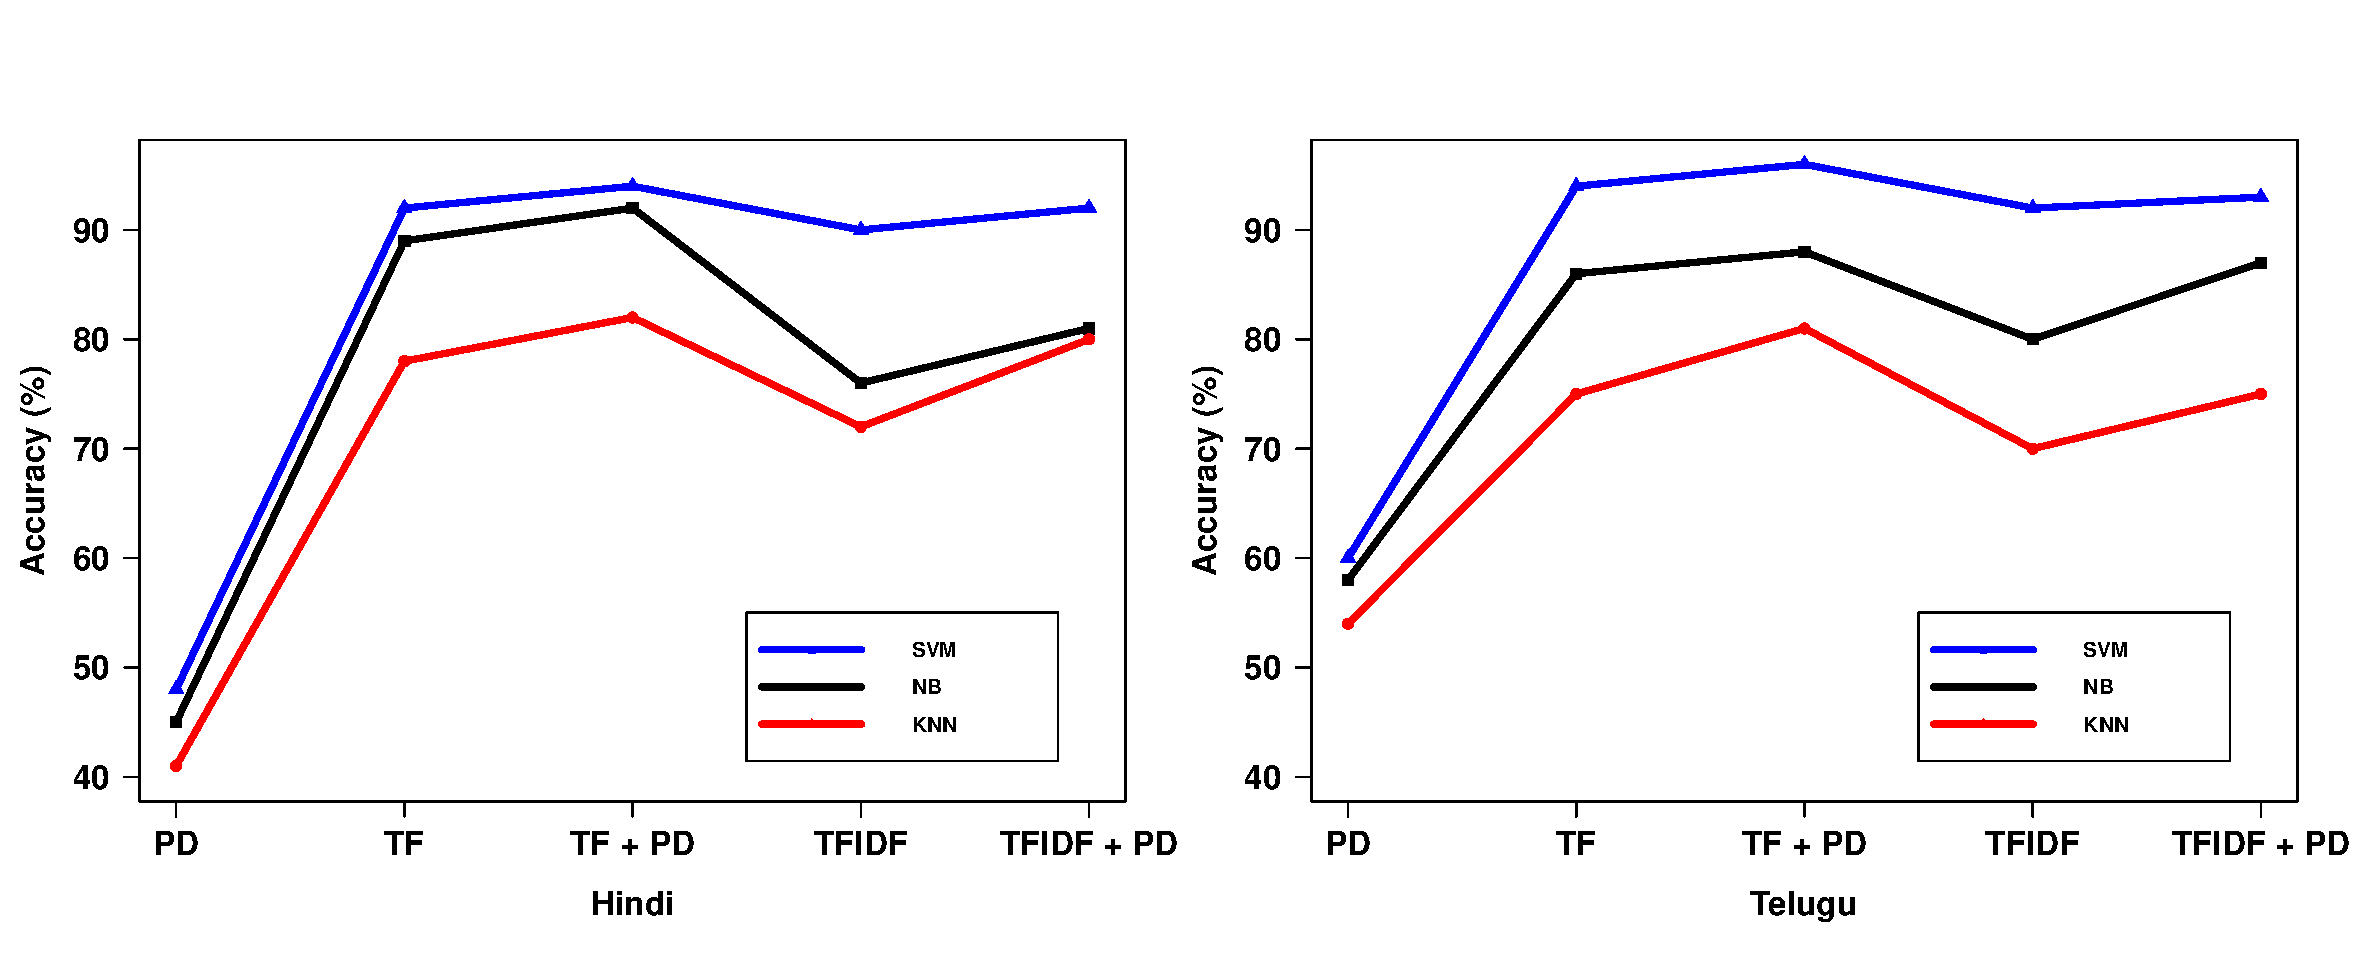
\includegraphics{figures/Story_Cln_90_set_2}}
\centering
\caption{Story classification accuracy using concatenation of keyword and POS features}
\label{Figure: Story Accuracy set 2}
\end{figure} 


\end{frame}
%%%%%%%%%%%%%%%%%%%%%%%%%%%%%%%%%%%%%%%%%%%%%%%%%%%%%%%%%%%%%%%%%%%%%%%%%%%%%%%%%%%%%%%%%


%%%%%%%%%%%%%%%%%%%%%%%%%%%%%%%%%%%%%%%%%%%%%%%%%%%%%%%%%%%%%%%%%%%%%%%%%%%%%%%%%%%%%%%%%
\begin{frame}
\frametitle{McNemar's Significance Test Results for Different Combinations of Features}

\begin{table}
\renewcommand{\arraystretch}{1}
\caption {Statistical significance test results for different combination of features \label{Table: Mcnemar result of significance test}}
\resizebox{\linewidth}{!}{
\begin{tabular}{|c|c|c||c|c|}
\hline
\multirow{2}{*}{Classifier} & \multicolumn{2}{c||}{Hindi} & \multicolumn{2}{c|}{Telugu} \\ \cline{2-5} 
 & TF + PD vs TF & TFIDF + PD vs TFIDF & TF + PD vs TF & TFIDF + PD vs TFIDF \\ \hline
NB & $>$ & $\sim$ & $>$ & $\sim$ \\ \hline
KNN & $\sim$ & $\sim$ & $\sim$ & $\sim$ \\ \hline
SVM & $>$ & $>$ & $>$ & $>$ \\ \hline
\end{tabular}}
\begin{threeparttable} 
	\begin{tablenotes} 
 `` $>$ " means 0.01 $<$ \textit{P-value} $\leq$ 0.05, which is statistically significant \\ `` $\sim$ " means \textit{P-value} $>$ 0.05, which is not statistically significant 
    \end{tablenotes}
  \end{threeparttable}

\end{table}	
\href{run:Mcnemar.pdf}{Demo}
\end{frame}
%%%%%%%%%%%%%%%%%%%%%%%%%%%%%%%%%%%%%%%%%%%%%%%%%%%%%%%%%%%%%%%%%%%%%%%%%%%%%%%%%%%%%%%%%


%%%%%%%%%%%%%%%%%%%%%%%%%%%%%%%%%%%%%%%%%%%%%%%%%%%%%%%%%%%%%%%%%%%%%%%%%%%%%%%%%%%%%%%%%
\begin{frame}
\frametitle{McNemar's Significance Test Results for Cross-classifier Performance}

\begin{table} 
\renewcommand{\arraystretch}{1}
\caption {Statistical significance test results for cross-classifier performance \label{Table: Cross classifier significance test}}
\resizebox{\linewidth}{!}{
\begin{tabular}{|c|c|c|c|c|c|c||c|c|c|c|c|}
\hline
\multirow{2}{*}{Classifier A} & \multirow{2}{*}{Classifier B} & \multicolumn{5}{c||}{Hindi} & \multicolumn{5}{c|}{Telugu} \\ \cline{3-12} 
 &  & PD & TF & TF + PD & TFIDF & TFIDF + PD & PD & TF & TF + PD & TFIDF & TFIDF + PD \\ \hline
NB & KNN & $\sim$ & $\gg$ & $\gg$ & $>$ & $\sim$ & $\sim$ & $\gg$ & $\gg$ & $\gg$ & $\gg$ \\ \hline
SVM & KNN & $\sim$ & $\gg$ & $\gg$ & $\gg$ & $\gg$ & $\sim$ & $\gg$ & $\gg$ & $\gg$ & $\gg$ \\ \hline
SVM & NB & $\sim$ & $\sim$ & $\sim$ & $\gg$ & $\gg$ & $\sim$ & $\gg$ & $>$ & $\gg$ & $>$ \\ \hline
\end{tabular}}
\begin{threeparttable} 
	\begin{tablenotes}
     `` $\gg$ " means \textit{P-value} $\leq$ 0.01, which is extremely statistically significant \\ `` $>$ " means 0.01 $<$ \textit{P-value} $\leq$ 0.05, which is statistically significant \\ `` $\sim$ " means \textit{P-value} $>$ 0.05, which is not statistically significant
    \end{tablenotes}
  \end{threeparttable}
\end{table} 
\href{run:Mcnemar.pdf}{Demo}
\end{frame}
%%%%%%%%%%%%%%%%%%%%%%%%%%%%%%%%%%%%%%%%%%%%%%%%%%%%%%%%%%%%%%%%%%%%%%%%%%%%%%%%%%%%%%%%%

%%%%%%%%%%%%%%%%%%%%%%%%%%%%%%%%%%%%%%%%%%%%%%%%%%%%%%%%%%%%%%%%%%%%%%%%%%%%%%%%%%%%%%%%%
\begin{frame} \label{Concatenation of keyword and POS}
\frametitle{Analysis of Results of Story Classification using Concatenation of Keyword and POS Features}

\begin{itemize}
\item[--] NB is a probabilistic learning method. It is based on Bayes theorem and the story genre will be assigned to the class having maximum a posteriori probability.
\item[--] The poor performance of KNN can be due to the noisy terms in the DTM.
\item[--] SVM has better performance because it is resilient to noise.
\end{itemize}

\hyperlink{Confusion Matrix}{\beamergotobutton{}} 

\end{frame}
%%%%%%%%%%%%%%%%%%%%%%%%%%%%%%%%%%%%%%%%%%%%%%%%%%%%%%%%%%%%%%%%%%%%%%%%%%%%%%%%%%%%%%%%%


\section{Summary and Conclusions}

\begin{frame}
\frametitle{Summary and Conclusions}
\begin{itemize}
\item[--] Contributions
\begin{itemize}
\item[--] Developed story corpora for Hindi and Telugu.
\item[--] Story Classification using Concatenation of Keyword and POS Features.
\end{itemize}
\item[--] Conclusions
\begin{itemize}
\item[--] In case of feature reduction techniques, sparseness factor of \textbf{0.9} gave the highest performance.
\item[--] Using linguistic information boosts the performance of story classification significantly.
\item[--] POS tag set consisting of nouns, adjectives and quantifiers have the highest accuracy and are important for story classification.
\item[--] In most of the cases, the highest performance is achieved by TF + PD features and SVM models outperformed the other models in terms of classification accuracy.
\end{itemize}
\end{itemize}
\end{frame}

%%%%%%%%%%%%%%%%%%%%%%%%%%%%%%%%%%%%%%%%%%%%%%%%%%%%%%%%%%%%%%%%%%%%%%%%%%%%%%%%%%%%%%%%%
\section{Future Work}
\begin{frame}
\frametitle{Future Work}
\begin{itemize}
\item[--] \textit{Story classification using partial story information:} Exploring story classification by dividing stories into parts based on story semantics.
\item[--] \textit{Emotion prediction from story text:} Exploring Keyword, POS and story specific features for predicting emotion from story text.
\item[--] \textit{Deriving prosody rules:} Deriving prosody rules (modification factors) specific to emotions and story genres.
\item[--] \textit{Synthesis of story speech using mark-up language:} Story-specific prosody rules can be effectively incorporated using SABLE mark-up language. The quality and naturalness of the synthesized story speech can be evaluated using subjective tests.
\end{itemize}
\end{frame}
%%%%%%%%%%%%%%%%%%%%%%%%%%%%%%%%%%%%%%%%%%%%%%%%%%%%%%%%%%%%%%%%%%%%%%%%%%%%%%%%%%%%%%%%%

%%%%%%%%%%%%%%%%%%%%%%%%%%%%%%%%%%%%%%%%%%%%%%%%%%%%%%%%%%%%%%%%%%%%%%%%%%%%%%%%%%%%%%%%%
\begin{frame}
\frametitle{Publications}
\label{Publications}
\begin{itemize}
\item \textbf{Conference}
	\begin{itemize}
	 	\item[--]  Harikrishna D M and K. Sreenivasa Rao, ``\textit{Classification of Children Stories in Hindi Using Keywords and POS Density,"} in \textit{International Conference on Computer Communication and Control (IC4)}, Indore, 2015. 
	 	\end{itemize}
\end{itemize}
\end{frame}
%%%%%%%%%%%%%%%%%%%%%%%%%%%%%%%%%%%%%%%%%%%%%%%%%%%%%%%%%%%%%%%%%%%%%%%%%%%%%%%%%%%%%%%%%

%%%%%%%%%%%%%%%%%%%%%%%%%%%%%%%%%%%%%%%%%%%%%%%%%%%%%%%%%%%%%%%%%%%%%%%%%%%%%%%%%%%%%%%%%
\begin{frame}
\frametitle{\begin{center}
ACKNOWLEDGMENTS
\end{center}}
\begin{center}
We are thankful to the \textbf{Department of Information Technology, Govt. of India} for supporting the research work, \textbf{``Development of Text-to-Speech synthesis for Indian Languages Phase II"}
\end{center}
\end{frame}
%%%%%%%%%%%%%%%%%%%%%%%%%%%%%%%%%%%%%%%%%%%%%%%%%%%%%%%%%%%%%%%%%%%%%%%%%%%%%%%%%%%%%%%%%



\begin{frame}[allowframebreaks]{References}    
\bibliographystyle{IEEEtran}    %apalike, plainnat, amsalpha, IEEEtran, ieeetr
\bibliography{Ref}
\end{frame}


\begin{frame}
\Huge{\centerline{Thank You}}
\end{frame}


%%%%%%%%%%%%%%%%%%%%%%%%%%%%%%%%%%%%%%%%%%%%%%%%%%%%%%%%%%%%%%%%%%%%%%%%%%%%%%%%%%%%%%%%%
\begin{frame}[noframenumbering]
\Huge{\centerline{Backup Slides}}
\end{frame}
%%%%%%%%%%%%%%%%%%%%%%%%%%%%%%%%%%%%%%%%%%%%%%%%%%%%%%%%%%%%%%%%%%%%%%%%%%%%%%%%%%%%%%%%%


\begin{frame}[noframenumbering] \label{McNemar's significance test}
\frametitle{McNemar's significance test}
\begin{itemize}
\item[--] Contingency table \\ 

\vspace{0.5cm}

\begin{tabular}{p{5cm}|p{5cm}}
\hline 
$\eta_{00}:$ Number of examples misclassified by both classifiers $C_A$ and $C_B$ & $\eta_{01}:$ Number of examples misclassified by classifier $C_A$ but not by $C_B$ \\ 
\hline 
$\eta_{10}:$ Number of examples misclassified by classifier $C_B$ but not by $C_A$  & $\eta_{11}:$ Number of examples misclassified by neither classifiers $C_A$ nor $C_B$ \\ 
\hline 
\end{tabular}
%\end{table}	

\vspace{0.5cm}

\item[--] The statistic $\chi$ is defined as 
\begin{equation*}
\chi = \frac{(\mid\eta_{01} - \eta_{10}\mid - 1)^2}{\eta_{01} + \eta_{10}}
\end{equation*}
\end{itemize}

\hyperlink{Evaluation Measures}{\beamerreturnbutton{}}

\end{frame}


%%%%%%%%%%%%%%%%%%%%%%%%%%%%%%%%%%%%%%%%%%%%%%%%%%%%%%%%%%%%%%%%%%%%%%%%%%%%%%%%%%%%%%%%%
\begin{frame}[noframenumbering] \label{Sparse Term Removal}
\frametitle{Sparse Term Removal Example}
\begin{figure}[h] 
\centering
\resizebox{10cm}{6cm}{\includegraphics{figures/text}}
\centering
\caption{Story text}
\label{DTM}
\end{figure}
\end{frame}
%%%%%%%%%%%%%%%%%%%%%%%%%%%%%%%%%%%%%%%%%%%%%%%%%%%%%%%%%%%%%%%%%%%%%%%%%%%%%%%%%%%%%%%%%


%%%%%%%%%%%%%%%%%%%%%%%%%%%%%%%%%%%%%%%%%%%%%%%%%%%%%%%%%%%%%%%%%%%%%%%%%%%%%%%%%%%%%%%%%
\begin{frame}[noframenumbering]
\frametitle{Document Term Matrix}
\begin{figure}[h] 
\centering
\resizebox{12cm}{6cm}{\includegraphics{figures/no_sparse}}
\centering
\caption{Document Term Matrix}
\label{DTM}
\end{figure}
\end{frame}
%%%%%%%%%%%%%%%%%%%%%%%%%%%%%%%%%%%%%%%%%%%%%%%%%%%%%%%%%%%%%%%%%%%%%%%%%%%%%%%%%%%%%%%%%

%%%%%%%%%%%%%%%%%%%%%%%%%%%%%%%%%%%%%%%%%%%%%%%%%%%%%%%%%%%%%%%%%%%%%%%%%%%%%%%%%%%%%%%%%
\begin{frame}[noframenumbering]
\frametitle{Sparse Term Removal}
\begin{itemize}
\item[--] Sparseness factor = 0.1
\item[--] Remove terms which have greater than 10\% percentage of empty elements or get terms which exists in 90\% of stories.
\end{itemize}
\begin{figure}[h] 
\centering
\resizebox{12cm}{5cm}{\includegraphics{figures/sparse_1}}
\centering
\caption{With Sparseness factor of 0.1}
\label{DTM}
\end{figure}
\end{frame}
%%%%%%%%%%%%%%%%%%%%%%%%%%%%%%%%%%%%%%%%%%%%%%%%%%%%%%%%%%%%%%%%%%%%%%%%%%%%%%%%%%%%%%%%%

%%%%%%%%%%%%%%%%%%%%%%%%%%%%%%%%%%%%%%%%%%%%%%%%%%%%%%%%%%%%%%%%%%%%%%%%%%%%%%%%%%%%%%%%%
\begin{frame}[noframenumbering]
\frametitle{Sparse Term Removal (Cont...)}
\begin{itemize}
\item[--] Sparseness factor = 0.2
\item[--] Remove terms which have greater than 20\% percentage of empty elements or get terms which exists in 80\% of stories.
\end{itemize}
\begin{figure}[h] 
\centering
\resizebox{12cm}{5cm}{\includegraphics{figures/sparse_2}}
\centering
\caption{With Sparseness factor of 0.2}
\label{DTM}
\end{figure}
\end{frame}
%%%%%%%%%%%%%%%%%%%%%%%%%%%%%%%%%%%%%%%%%%%%%%%%%%%%%%%%%%%%%%%%%%%%%%%%%%%%%%%%%%%%%%%%%

%%%%%%%%%%%%%%%%%%%%%%%%%%%%%%%%%%%%%%%%%%%%%%%%%%%%%%%%%%%%%%%%%%%%%%%%%%%%%%%%%%%%%%%%%
\begin{frame}[noframenumbering]
\frametitle{Sparse Term Removal (Cont...)}
\begin{itemize}
\item[--] Sparseness factor = 0.4
\item[--] Remove terms which have greater than 40\% percentage of empty elements or get terms which exists in 60\% of stories.
\end{itemize}
\begin{figure}[h] 
\centering
\resizebox{12cm}{5cm}{\includegraphics{figures/sparse_4}}
\centering
\caption{With Sparseness factor of 0.4}
\label{DTM}
\end{figure}
\end{frame}
%%%%%%%%%%%%%%%%%%%%%%%%%%%%%%%%%%%%%%%%%%%%%%%%%%%%%%%%%%%%%%%%%%%%%%%%%%%%%%%%%%%%%%%%%

%%%%%%%%%%%%%%%%%%%%%%%%%%%%%%%%%%%%%%%%%%%%%%%%%%%%%%%%%%%%%%%%%%%%%%%%%%%%%%%%%%%%%%%%%
\begin{frame}[noframenumbering]
\frametitle{Sparse Term Removal (Cont...)}
\begin{itemize}
\item[--] Sparseness factor = 0.9. \hyperlink{Story Classification using Keyword based Features}{\beamerreturnbutton{}}
\item[--] Remove terms which have greater than 90\% percentage of empty elements or get terms which exists in 10\% of stories.
\item[--] Same as without sparse term removal
\end{itemize} 
\begin{figure}[h] 
\centering
\resizebox{12cm}{5cm}{\includegraphics{figures/sparse_9}}
\centering
\caption{With Sparseness factor of 0.9}
\label{DTM}
\end{figure}

\end{frame}
%%%%%%%%%%%%%%%%%%%%%%%%%%%%%%%%%%%%%%%%%%%%%%%%%%%%%%%%%%%%%%%%%%%%%%%%%%%%%%%%%%%%%%%%%

%%%%%%%%%%%%%%%%%%%%%%%%%%%%%%%%%%%%%%%%%%%%%%%%%%%%%%%%%%%%%%%%%%%%%%%%%%%%%%%%%%%%%%%%%
\begin{frame}[noframenumbering] \label{LSA} 
\frametitle{Latent Semantic Analysis}
\begin{itemize}
\item[--] Basic Idea: Let $C$ be a DTM $(M \times N)$ with non-negative real valued entries and $m = min(M,N)$. $C$ can be decomposed into a set of $k$ orthogonal matrices whose linear combination is a good approximation of initial matrix $C$.
\item[--] Formal definition: $C$ can be decomposed as, $C = U S V^T$; where matrices $U (M \times m)$ and $V (N \times m)$ are orthonormal matrices ($U^TU = I_m$ and $V^TV = I_m$) whose columns define left and right singular vectors respectively and $S$ is a $m \times m$ diagonal matrix of singular values of $C$ decreasingly ordered along its diagonal. 

\item[--] Retain only the $k$ greatest singular values in $S$ ,then the product of resulting matrices $S_k$, $U_k$ and $V_k$ is the best approximation of original $C$ by a matrix of rank $k$

\begin{equation*}
\title{LSA_normalised}
C \simeq C_k = U_k S_k V_k^T
\end{equation*}

where $C_k$ is the approximation of original document-term matrix $C$, $S_k$ is a diagonal matrix consisting of largest $k$ values.

\end{itemize} 

\end{frame}
%%%%%%%%%%%%%%%%%%%%%%%%%%%%%%%%%%%%%%%%%%%%%%%%%%%%%%%%%%%%%%%%%%%%%%%%%%%%%%%%%%%%%%%%%

%%%%%%%%%%%%%%%%%%%%%%%%%%%%%%%%%%%%%%%%%%%%%%%%%%%%%%%%%%%%%%%%%%%%%%%%%%%%%%%%%%%%%%%%%
\begin{frame}[noframenumbering] 
\frametitle{LSA Example}
\begin{itemize}
\item[--] Source: Introduction to Information Retrieval (Manning et al., 2008)
\item[--] Consider a term-document matrix $C$
\end{itemize}
\begin{figure}[h] 
\centering
\resizebox{5cm}{2.3cm}{\includegraphics{figures/dtm}}
\centering
\caption{Term document matrix}
\label{DTM_LSA}
\end{figure}

\begin{itemize}
\item[--] Matrix $U$
\end{itemize}
\begin{figure}[h] 
\centering
\resizebox{4cm}{1.5cm}{\includegraphics{figures/u_matrix}}
\centering
\caption{SVD term matrix}
\label{U_LSA}
\end{figure}

\end{frame}


%%%%%%%%%%%%%%%%%%%%%%%%%%%%%%%%%%%%%%%%%%%%%%%%%%%%%%%%%%%%%%%%%%%%%%%%%%%%%%%%%%%%%%%%%
\begin{frame}[noframenumbering]
\frametitle{LSA Example (Cont...)}

\begin{itemize}
\item[--] Matrix $S$
\end{itemize}
\begin{figure}[h] 
\centering
\resizebox{4cm}{2cm}{\includegraphics{figures/sigma}}
\centering
\caption{Singular Values matrix}
\label{Singular_LSA}
\end{figure}

\begin{itemize}
\item[--] Matrix $V^T$
\end{itemize}
\begin{figure}[h] 
\centering
\resizebox{4cm}{2cm}{\includegraphics{figures/v_matrix}}
\centering
\caption{SVD document matrix}
\label{VT_LSA}
\end{figure}

\end{frame}
%%%%%%%%%%%%%%%%%%%%%%%%%%%%%%%%%%%%%%%%%%%%%%%%%%%%%%%%%%%%%%%%%%%%%%%%%%%%%%%%%%%%%%%%%

%%%%%%%%%%%%%%%%%%%%%%%%%%%%%%%%%%%%%%%%%%%%%%%%%%%%%%%%%%%%%%%%%%%%%%%%%%%%%%%%%%%%%%%%%
\begin{frame}[noframenumbering]
\frametitle{LSA Example (Cont...)}

\begin{itemize}
\item[--] When $k = 2$, Matrix $S$
\end{itemize}
\begin{figure}[h] 
\centering
\resizebox{4cm}{2cm}{\includegraphics{figures/sigma_2}}
\centering
\caption{Singular Values matrix for k = 2}
\label{Sigma_2_LSA}
\end{figure}

\begin{itemize}
\item[--] Matrix $C_2$
\end{itemize}
\begin{figure}[h] 
\centering
\resizebox{4cm}{2cm}{\includegraphics{figures/c_2}}
\centering
\caption{Term document matrix for k = 2}
\label{C_2_LSA}
\end{figure}

\end{frame}
%%%%%%%%%%%%%%%%%%%%%%%%%%%%%%%%%%%%%%%%%%%%%%%%%%%%%%%%%%%%%%%%%%%%%%%%%%%%%%%%%%%%%%%%%


%%%%%%%%%%%%%%%%%%%%%%%%%%%%%%%%%%%%%%%%%%%%%%%%%%%%%%%%%%%%%%%%%%%%%%%%%%%%%%%%%%%%%%%%%
\begin{frame}[noframenumbering]
\frametitle{LSA Example (Cont...)}


\begin{itemize}
\item[--] Term document matrix $C$ reduced to two dimensions. \hyperlink{Story Classification using Keyword based Features}{\beamerreturnbutton{}}
\end{itemize}
\begin{figure}[h] 
\centering
\resizebox{8cm}{6cm}{\includegraphics{figures/dimension}}
\centering
\caption{Term document matrix reduced to two dimensions}
\label{Dimension_Reduction_LSA}
\end{figure}

\end{frame}


\begin{frame}[noframenumbering] \label{LSA Analysis} 
\frametitle{LSA Result Analysis}
\begin{itemize}
\item[--] LSA captures most of underlying structure in association of terms and documents.
\item[--] Since $k \ll terms$, it is expected that terms which occur in similar stories will be near each other in $k$ dimensional space even though if they never co-occur in same stories.
\item[--] Some stories which do not share any words in common, may however be near in $k-dimensional$ space.

\hyperlink{Keyword Result Analysis}{\beamerreturnbutton{}}
\end{itemize}
\end{frame}





\begin{frame}[noframenumbering] \label{Confusion Matrix} 
\frametitle{Confusion Matrix}
\begin{itemize}
\item[--] Confusion matrix for various classifiers using TF + PD features for Hindi. (A) indicates actual and (P) indicates predicted. \hyperlink{Concatenation of keyword and POS}{\beamerreturnbutton{}}

\begin{table}
\caption{Confusion matrix for NB}
\resizebox{6cm}{!}{
\begin{tabular}{|c|c|c|c|}
\hline
 & Fable (P) & Folk-tale (P) & Legend (P) \\ \hline
Fable (A) & 88 & 8 & 4 \\ \hline
Folk-tale (A) & 9 & 89 & 2 \\ \hline
Legend (A) & 5 & 5 & 90 \\ \hline
\end{tabular}}
\end{table}

\begin{table}
\caption{Confusion matrix for KNN}
\resizebox{6cm}{!}{
\begin{tabular}{|c|c|c|c|}
\hline
 & Fable (P) & Folk-tale (P) & Legend (P) \\ \hline
Fable (A) & 68 & 25 & 7 \\ \hline
Folk-tale (A) & 13 & 80 & 7 \\ \hline
Legend (A) & 6 & 4 & 90 \\ \hline
\end{tabular}}
\end{table}

\begin{table}
\caption{Confusion matrix for SVM}
\resizebox{6cm}{!}{
\begin{tabular}{|c|c|c|c|}
\hline
 & Fable (P) & Folk-tale (P) & Legend (P) \\ \hline
Fable (A) & 92 & 2 & 6 \\ \hline
Folk-tale (A) & 2 & 90 & 8 \\ \hline
Legend (A) & 3 & 4 & 93 \\ \hline
\end{tabular}}
\end{table}


\end{itemize}
\end{frame}




%----------------------------------------------------------------------------------------

\end{document} 
